%!TEX program = xelatex
\documentclass[titlepage,11pt,a4paper]{article}
\usepackage{amssymb}
\usepackage{dsfont}
\usepackage{graphicx}
\usepackage[ruled,vlined]{algorithm2e}
\graphicspath{ {results/} }
\usepackage[titlepage]{polytechnique}
\usepackage{subfig}


\title[INF 431 Programming Project]{Set multijoueurs}
    %\subtitle{Le sous-titre (optionnel, enlever cette ligne sinon)}
    \author{Zuli \textsc{HUANG}\\
            Yunxiang \textsc{ZHANG}
            }
    \date{06/04/2017}

\begin{document}
\maketitle

\section{Application à un joueur}

Dans un premier temps, nous avons développé une application pour un joueur seul sous Android. Le joueur peut choisir son propre compte pour accéder au jeu. Dans la graphe \ref{fig:login_screen_figure}, nous proposons au joueur deux genres de jeu. C'est-à-dire en ligne et off ligne. Par défaut, le choix est mis à \texttt{Offline Mode}. Nous commençons le jeu par cliquer \texttt{START}.\\


\begin{figure}[h]
\centering
\subfloat[Login Screen]{
  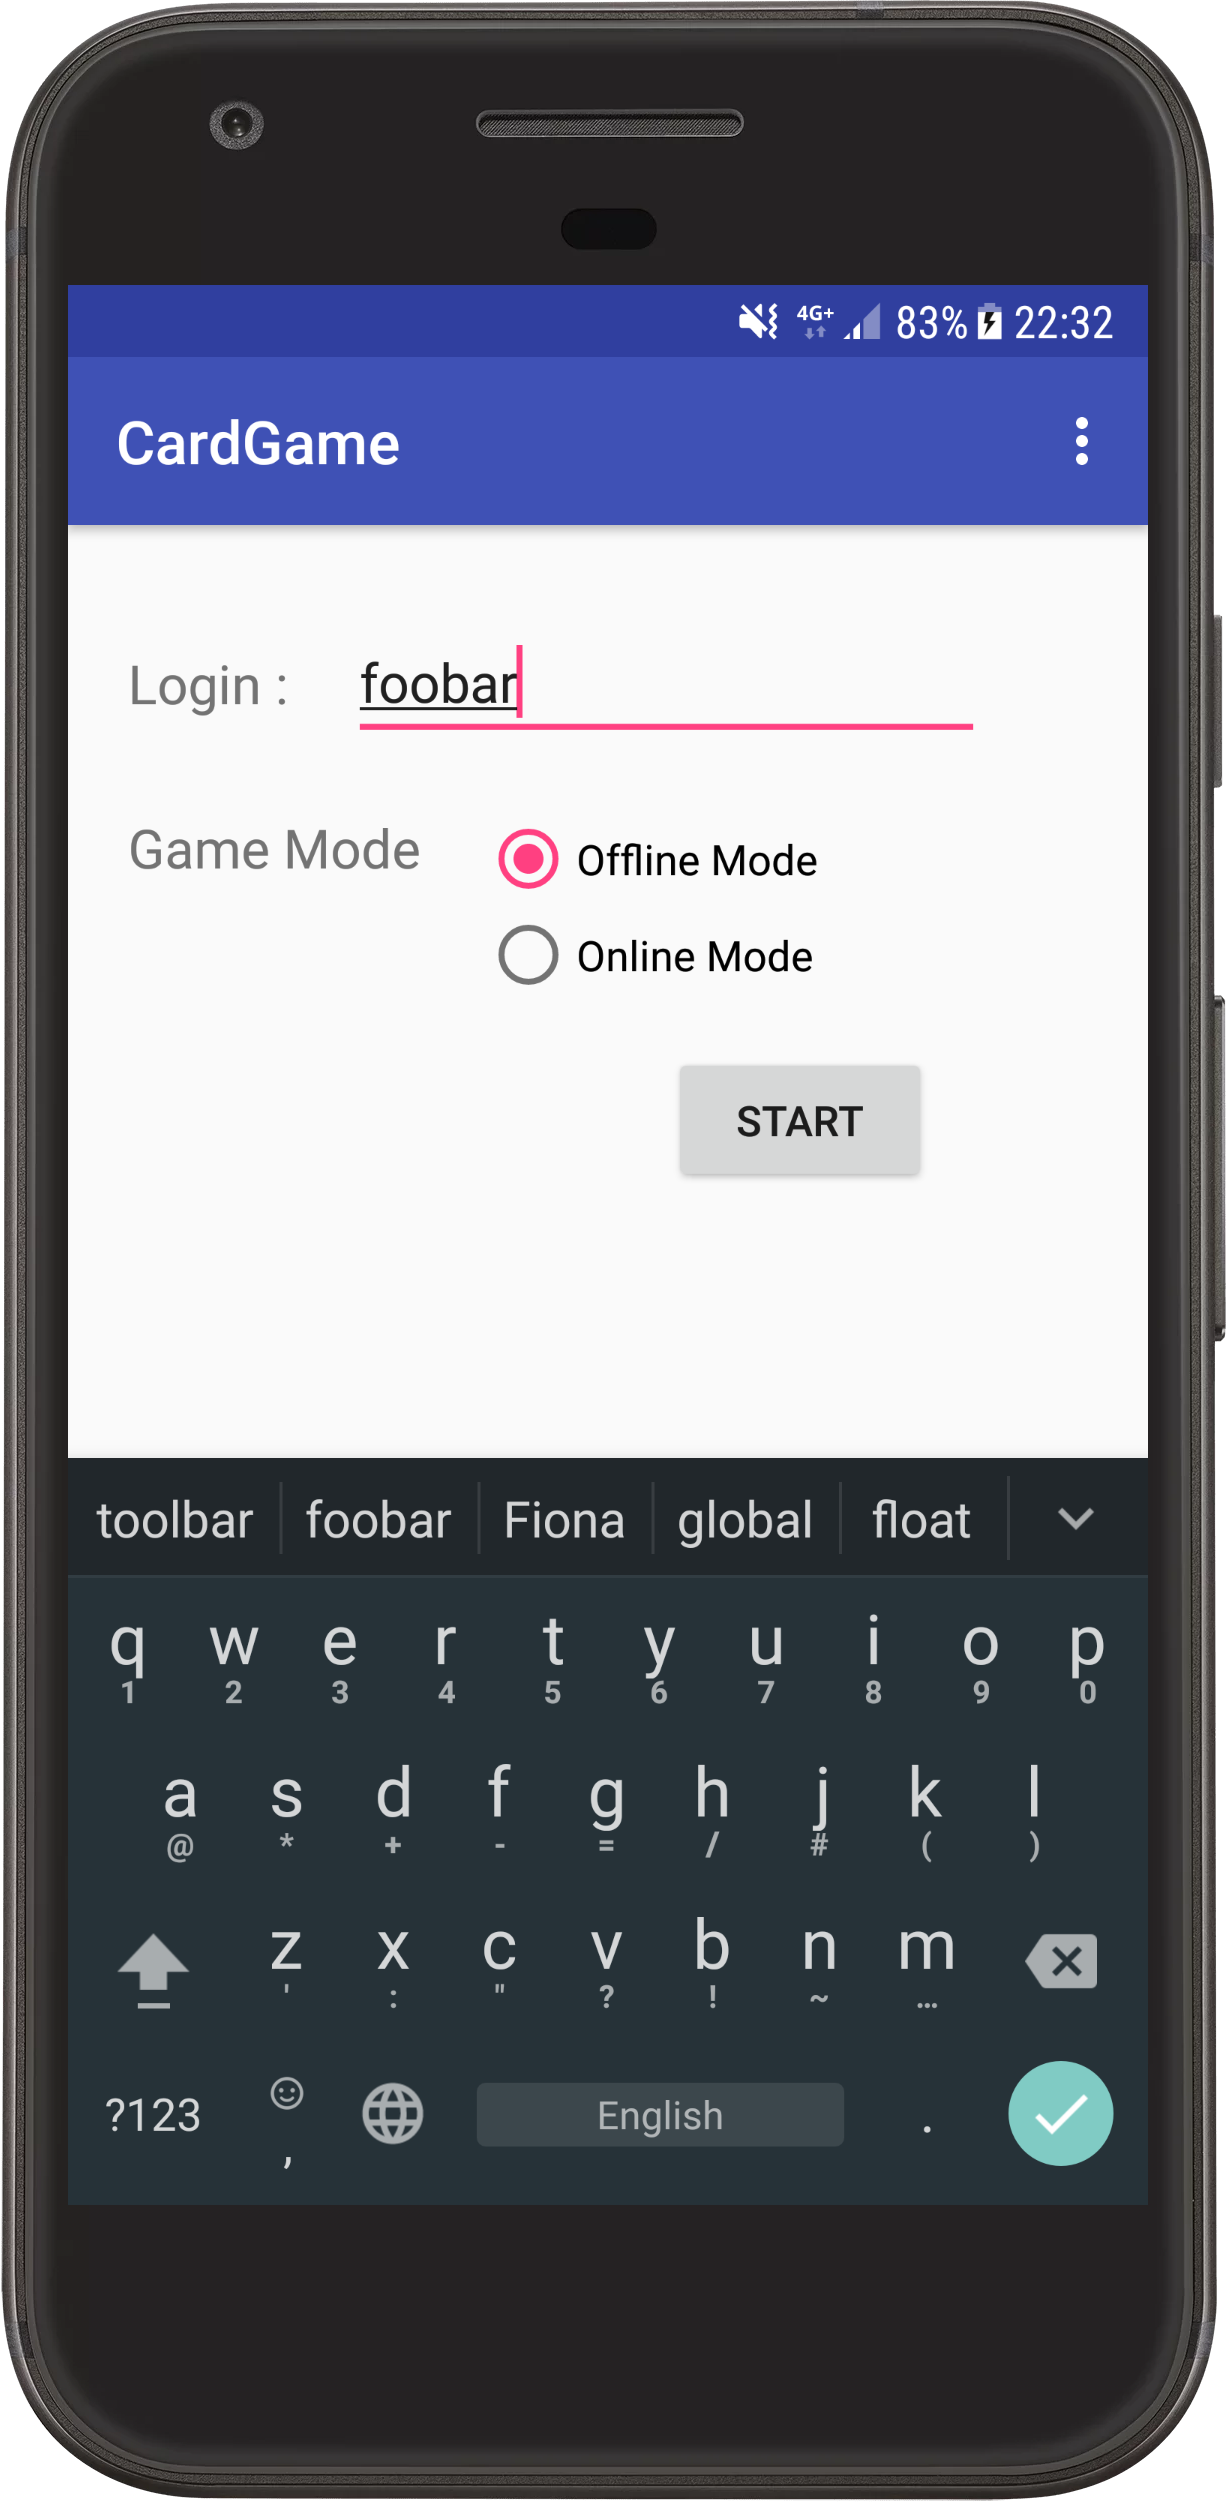
\includegraphics[height=13cm]{login_screen.png}
  \label{fig:login_screen_figure}
}
\subfloat[Main Game Screen]{
  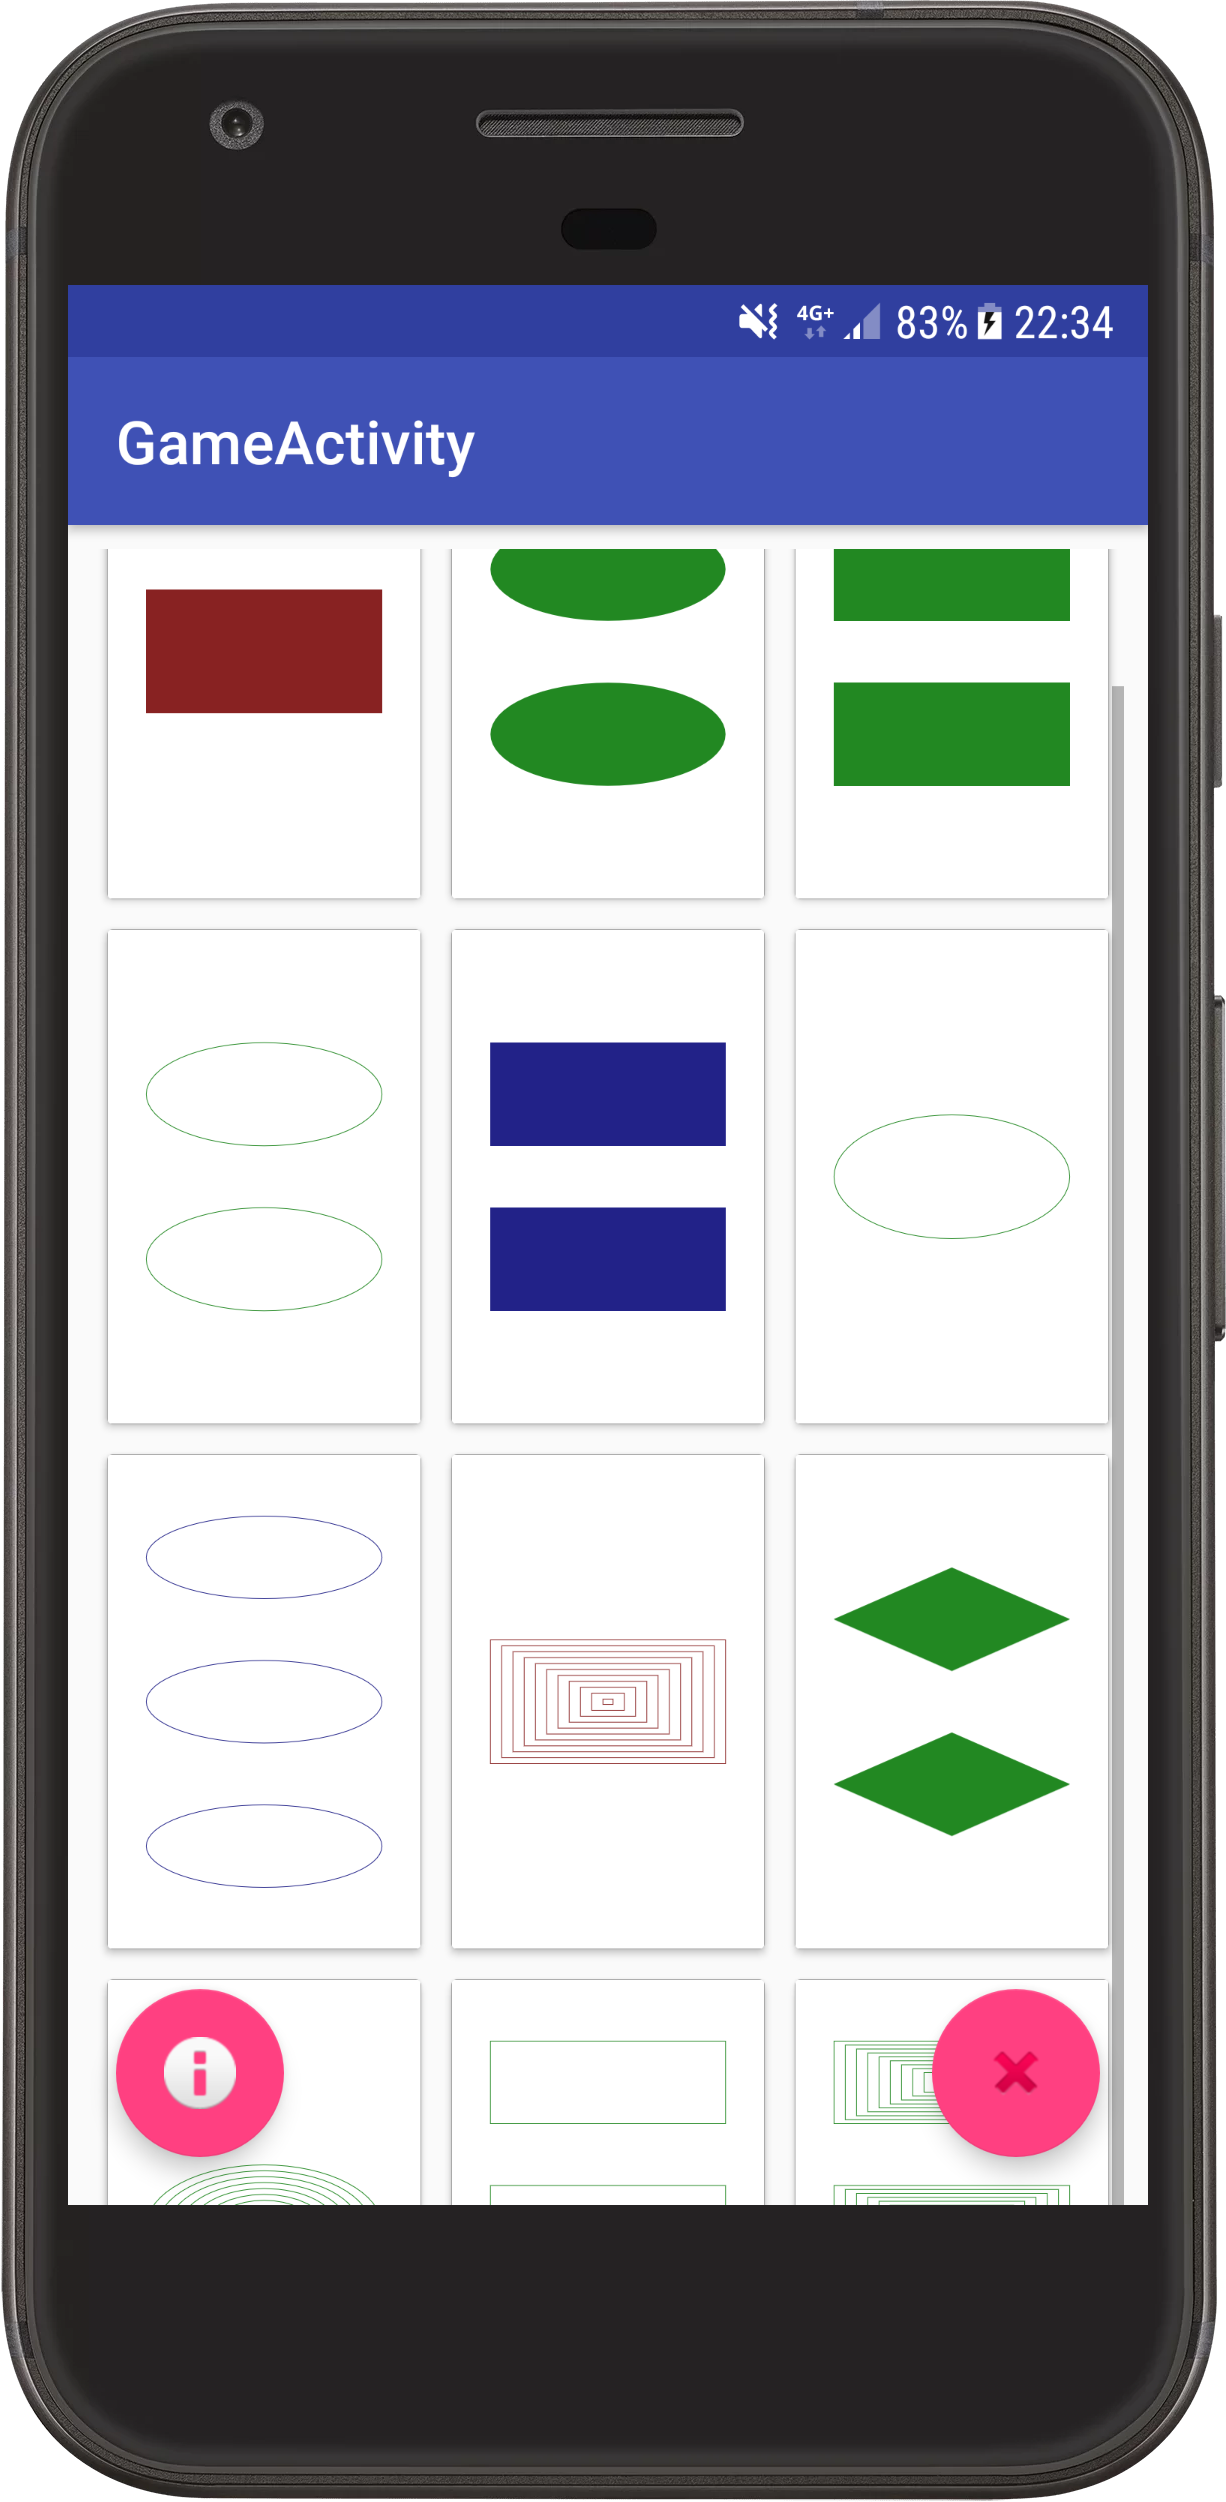
\includegraphics[height=13cm]{main_game_screen.png}
  \label{fig:main_game_figure}
}
\end{figure}
Dans cette interface graphique, nous avons utilisé un \texttt{OnClickListener} pour le bouton \texttt{START} pour que l'application réagisse à l'appuie de l'utilisateur.

Puis nous entrons au jeu, initialement, il y a 12 cartes. Nous avons conçu également un algorithme simple pour vérifier s'il existe un set dans toutes les cartes. Sinon, le système ajoutera automatiques 3 cartes. Par hypothèse, il existe toujours un set parmi 15 cartes. Le joueur peut choisir ses cartes par cliquer celles qui sont affichées. Il peut choisir 3 cartes au maximum. Au-delà de trois cartes, le programme l'empêchera à choisir les cartes.

Notammant, nous avons associé un \texttt{OnClickListener} pour chaque carte affiché sur l'écran. Suite à tous les changement d'état d'une carte, nous changeons sa couleur du fond. Puis, nous notifions à l'adapter des cartes affichables les changements. Enfin, l'application raffraîchit l'affichage.
\begin{figure}[h]
\centering
\subfloat[Choisir les cartes]{
  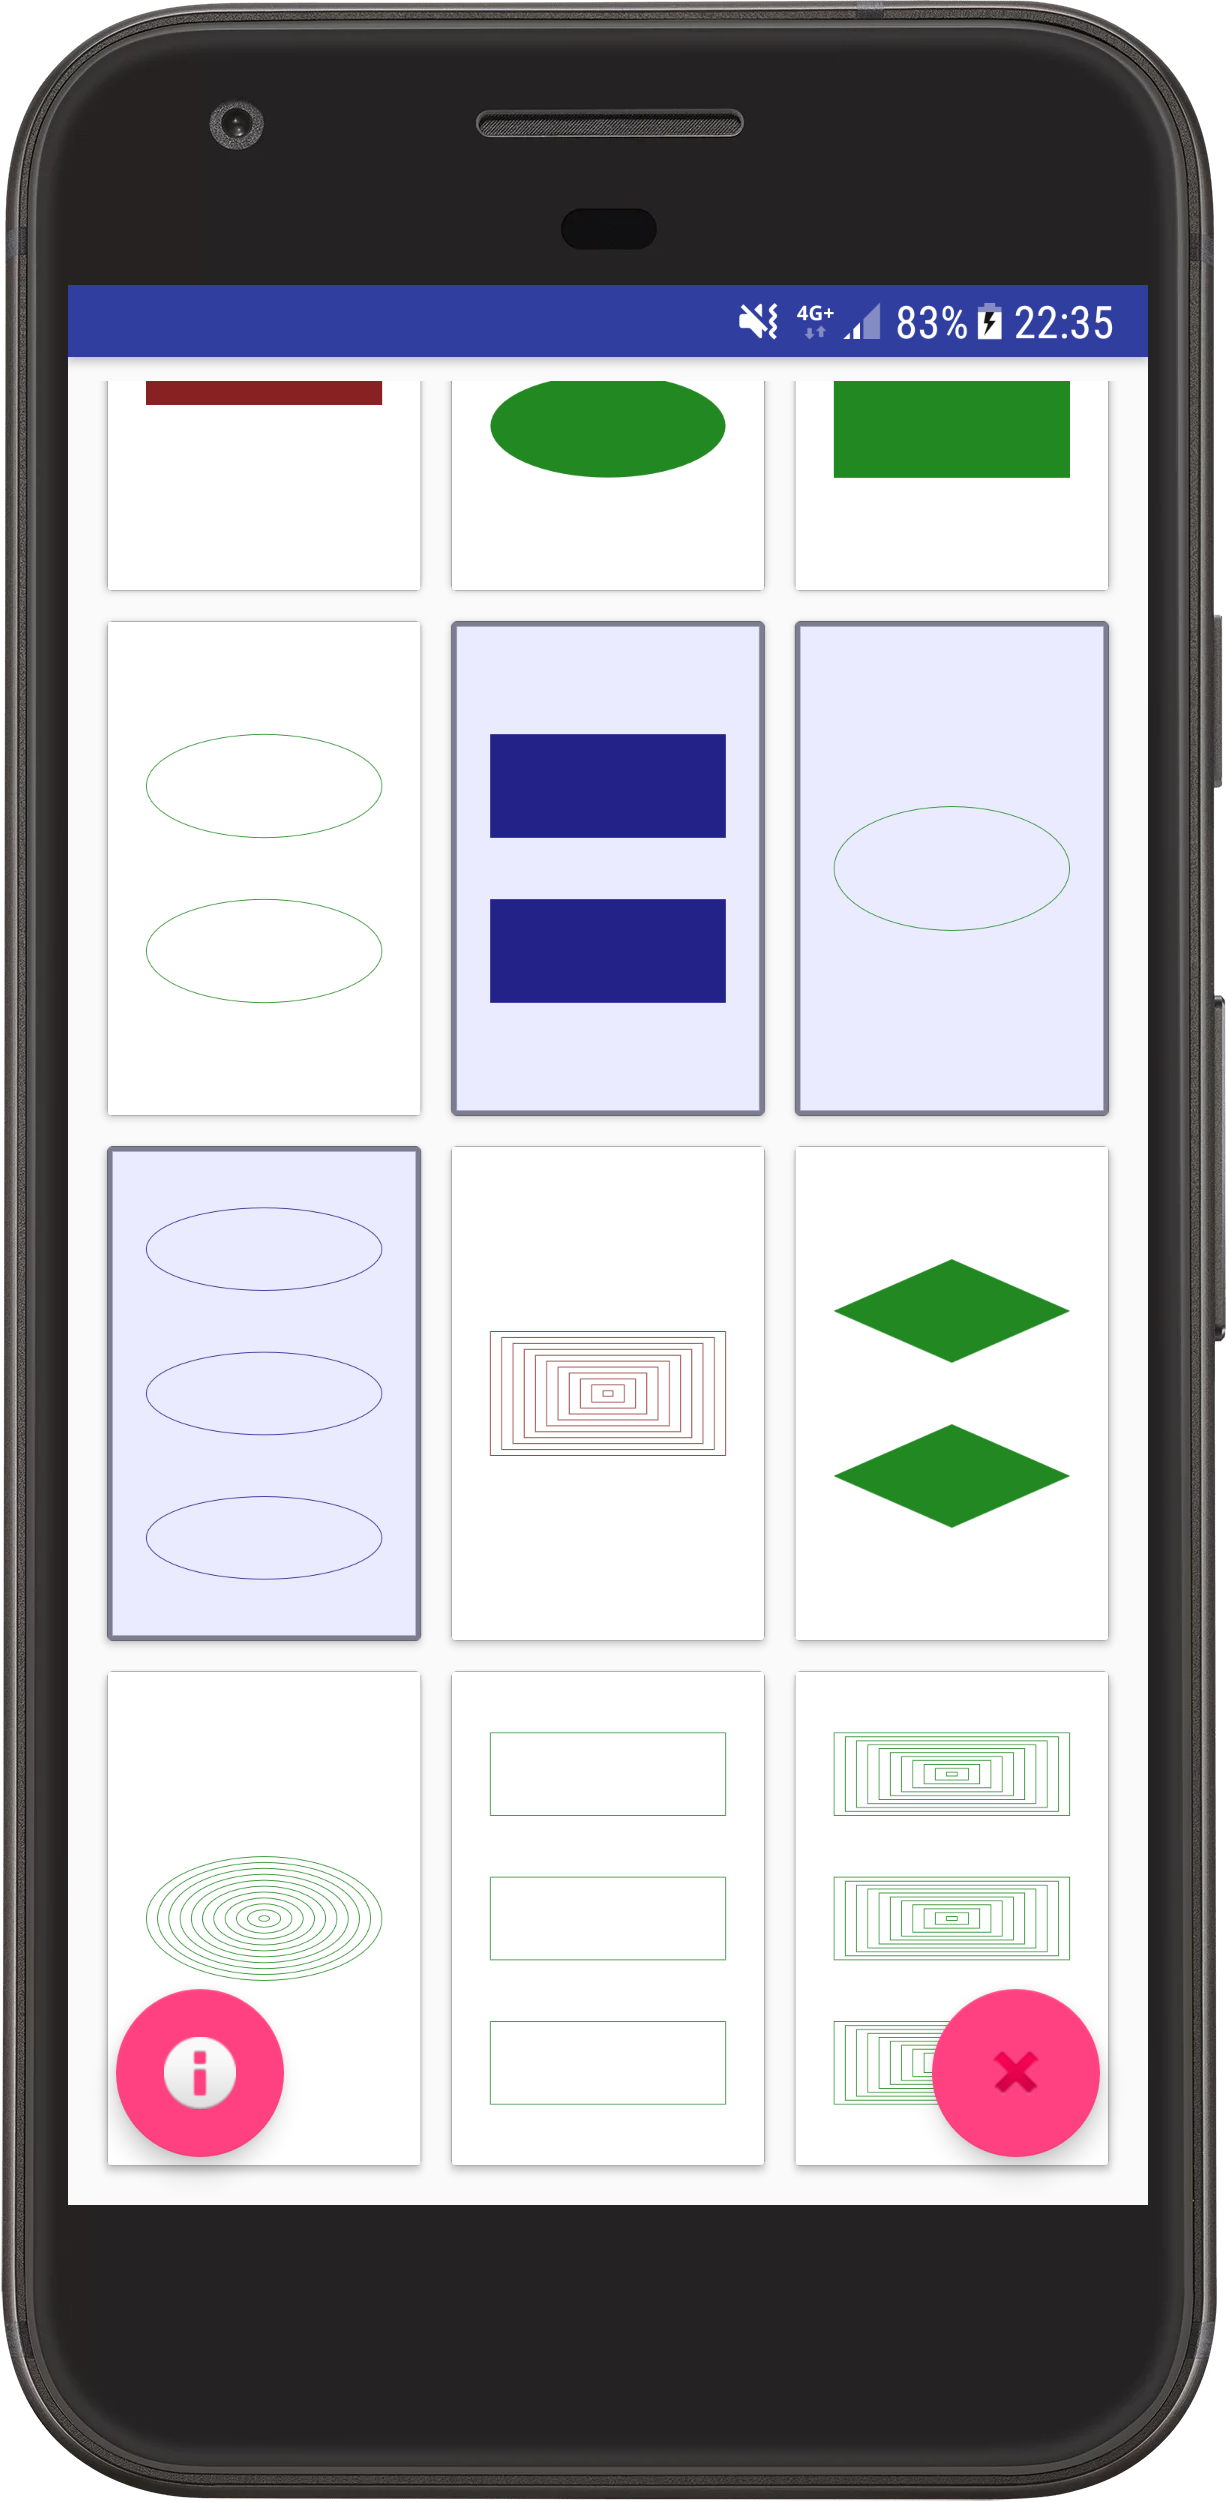
\includegraphics[height=13cm]{click_items_screen_shot.png}
  \label{fig:click_items_figure}
}
\subfloat[Points gagnés]{
  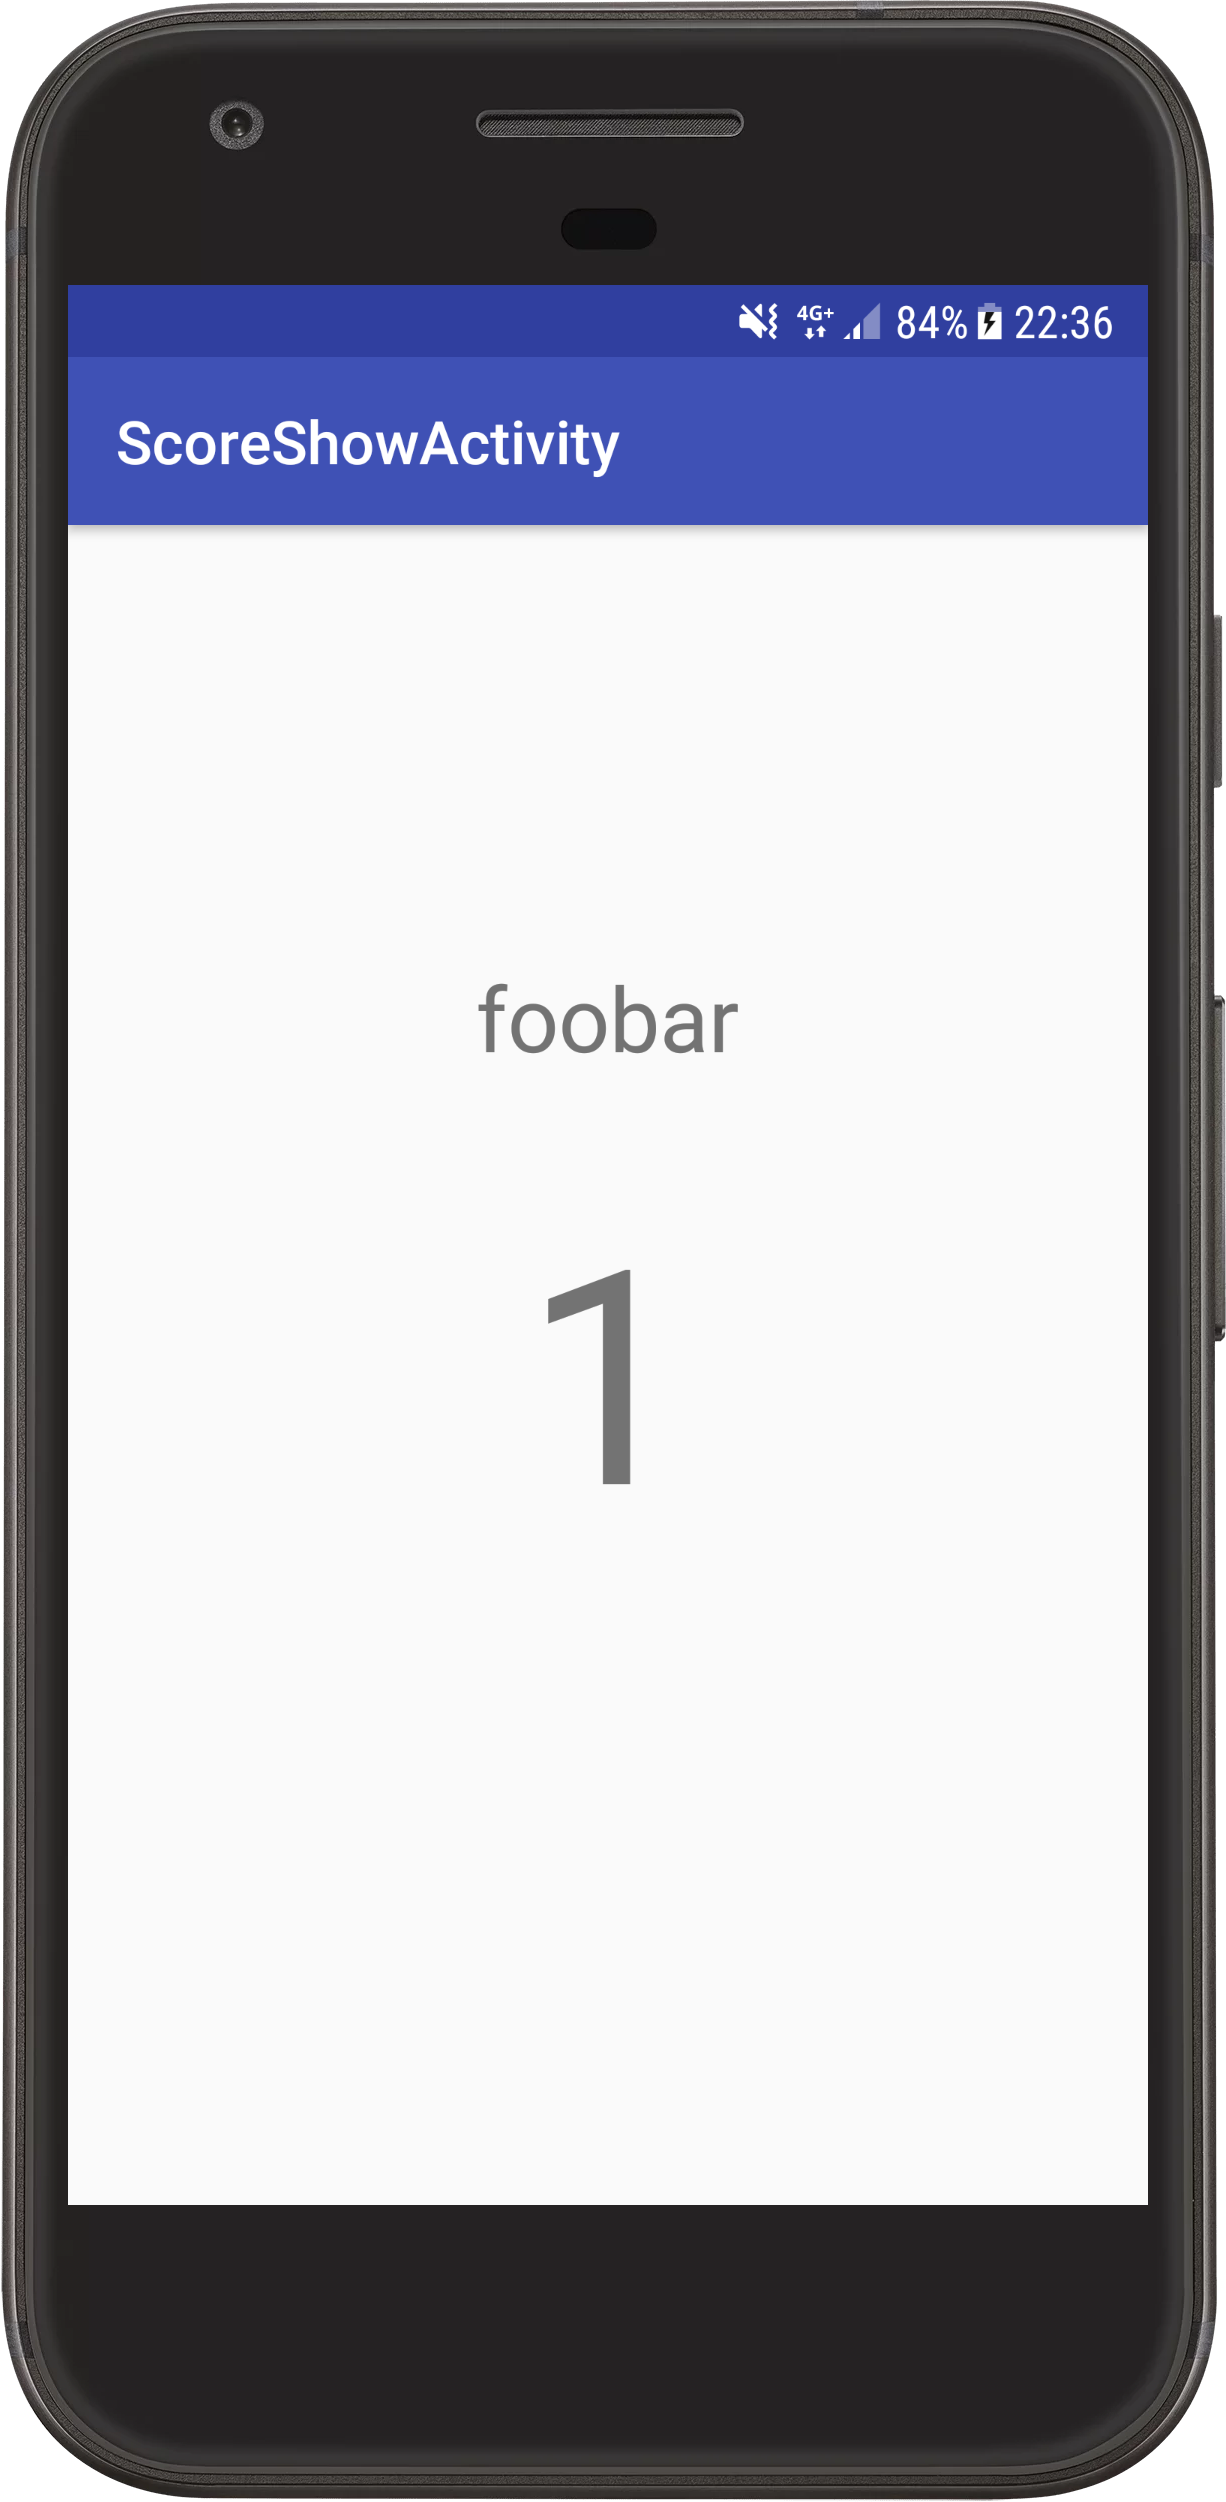
\includegraphics[height=13cm]{score_screen_shot.png}
  \label{fig:score_screen_figure}
}
\end{figure}

En cliquant le bouton rouge avec une croix, le programme vérifie si les cartes choisies par le joueur sont un set valid. Par taper le bouton rouge avec un point d'exlamation au milieu, nous afficherons les points que ce jour gagne. C'est-à-dire, nous l'associons aussi un \texttt{OnClickListener}. Ce listener evoquera l'affichage d'activité qui nous montre les points. Aprés chaque élimination, nous vérifions également s'il existe encore des sets valids.

\section{Implémentation Multijoueurs}
Nous avons choisit de mettre le serveur dans un ordinateur. Le serveur s'occupe d'abord d'initialiser les cartes qui seront distribuées aux joueurs. Puis, nous ouvrons un thread qui accepte la demande envoyée par les terminaux de joueurs. Une fois que nous recevons une demande, nous l'acceptons, et initialisons un thread pour chaque joueur afin de recevoir les messages. Nous avons deux sections critiques dans lesquelles nous ajoutons et retirons les cartes. Nous utilisons \texttt{lock()} et \texttt{unlock()} pour synchroniser les demandes envoyées par les joueurs.

Le serveur reçoit des commandes de clients. Un client qui reçoit uniquement des messages de serveur.

\begin{figure}[h]
\centering
\subfloat[Serveur]{
  \centering
  \includegraphics[height=7cm]{server_sreen_shot.png}
  \label{fig:server_sreen_figure}
}
\subfloat[Fake Client]{
  \centering
  \includegraphics[height=7cm]{fake_client_screen_shot.png}
  \label{fig:fake_client_figure}
}
\end{figure}

Et les comportements au portable.
\begin{figure}[h]
\centering
\subfloat[Online login]{
  \includegraphics[height=7.5cm]{online_login.png}
  \label{fig:online_login_figure}
}
\subfloat[Online click]{
  \includegraphics[height=7.5cm]{online_click_cards.png}
  \label{fig:online_click_figure}
}
\end{figure}

\end{document}
